\documentclass[14pt]{extreport}
\usepackage{gost}
\usepackage{longtable}
%Тут можно вставить дополнительные пакеты

\begin{document}
\pagestyle{empty} %  выключаем нумерацию

\includepdf[pages=-,pagecommand={}]{TitulList.pdf}

\pagestyle{plain} % включаем нумерацию
\tableofcontents

\intro

Целью данной практической работы является знакомством с LaTeX, а именно написание математического текста с формулами и рисунками, а также составлении таблиц.

\chapter{МАТЕМАТИЧЕСКИЙ ТЕКСТ\label{chapter2}}
\section{Пример математического текста}

Пусть на плоскости задана прямоугольная система координат. Комплексное число $z=a+bi$ изображается точкой на плоскости с координатами $(a, b)$, и эта точка обозначается той же буквой $z$ (рисунок ~\ref{fig1}). Действительные числа изображаются точками оси абсцисс (её называют действительной осью), а чисто мнимые числа - точками оси ординат (ее называют мнимой осью). Плоскость, на которой изображаются комплексные числа, называют комплексной плоскостью.
\begin{figure}[H]
\centerline{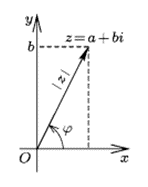
\includegraphics[width=0.25\linewidth]{pic1}}
\caption{Изображение комплексного числа $z=a+bi$ на плоскости}
\label{fig1}
\end{figure}
Комплексному числу $z=a+bi$ можно сопоставить вектор с началом в точке $O$ и концом в точке $z$ (рисунок ~\ref{fig1}). Этот вектор будем обозначать той же буквой $z$, его длина равна $|z|$.

Число $z_1 + z_2$ изображается вектором, построенным по правилу сложению векторов $z_1$ и $z_2$ (рисунок ~\ref{fig2}), а вектор $z_1 - z_2$ можно построить как сумму векторов $z_1$ и $-z_2$.
\begin{figure}[H]
\centerline{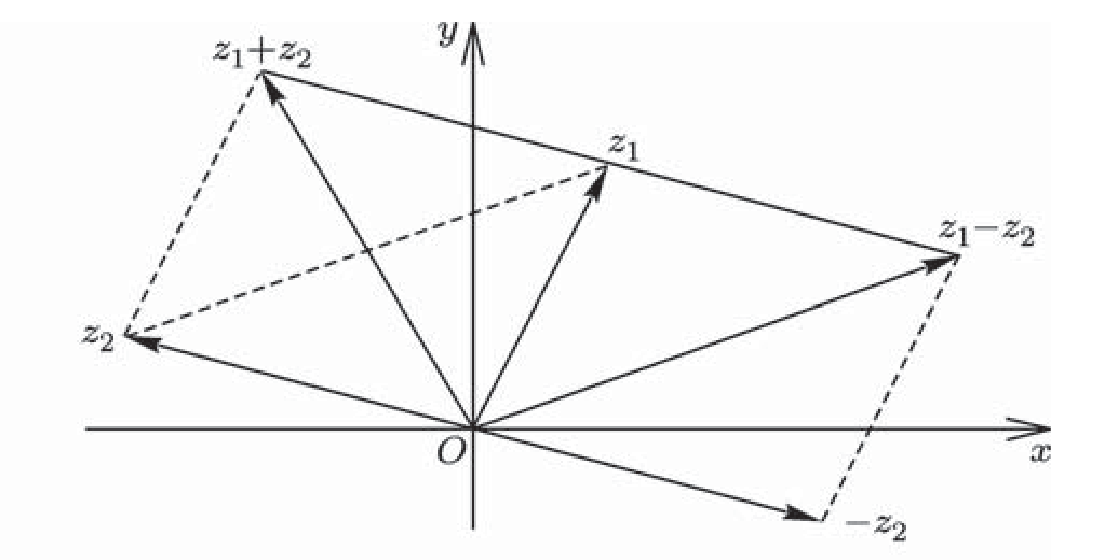
\includegraphics[width=0.5\linewidth]{pic2}}
\caption{Изображение чисел $z_1 + z_2$ и $z_1 - z_2$ на плоскости}
\label{fig2}
\end{figure}

Аргументом комплексного числа $z \neq 0$ называется угол $\varphi$ между положительным направлением действительной оси и вектором $z$ (рисунок~\ref{fig1}). Этот угол считается положительным, если отсчет угла ведется против часовой стрелки, и отрицательным – при отсчете по часовой стрелке.

Расстояние между точками $z_1$ и $z_2$ равно длине вектора $z_1 - z_2$, т. е. 
\begin{eqnarray*}
 |z_1 - z_2| = \sqrt{(a_1 - a_2)^2 + (b_1 - b_2)^2},
\end{eqnarray*}
где $z_1 = a_1 + b_1i, z_2 = a_2 + b_2i$.

Условию $|z - z_0| = R$, где $z_0$ - заданное комплексное число, $R>0$, удовлетворяют точки, лежащие на окружности радиуса $R$ с центром в точке $z_0$.

Для любых комплексных чисел $z_1, z_2$ справедливы неравенства
\begin{eqnarray*}
 |z_1 \pm z_2| <= |z_1| + |z_2|, |z_1 \pm z_2| >= ||z_1| - |z_2||
\end{eqnarray*}

Аргумент комплексного числа $z=a+bi (z\neq0)$ можно найти, решив систему ~(\ref{l2}). Эта система имеет бесконечно много решений вида $\varphi=\varphi_0+2k\pi$, где $k \in Z$, $\varphi_0$ – одно из решений системы ~(\ref{l2}), т. е. аргумент комплексного числа определяется неоднозначно.

Связь между действительной и мнимой частями комплексного числа $z=a+bi$ и его модулем $r=|z|$ и аргументом $\varphi$ выражается следующими формулами:
\begin{eqnarray}
 \begin{cases}
   a=r\cos\varphi \\
   b=r\sin\varphi
 \end{cases}
 \label{l1}
\end{eqnarray}
\begin{eqnarray}
 \begin{cases}
   \cos\varphi=\frac{a}{(\sqrt{a^2+b^2}} \\
   \cos\varphi=\frac{b}{(\sqrt{a^2+b^2}}
 \end{cases}
 \label{l2}
\end{eqnarray}

Для нахождения аргумента комплексного числа $z=a+bi (a\neq0)$ можно воспользоваться формулой
\begin{eqnarray}
\tg\varphi = \frac{b}{a}
 \label{l3}
\end{eqnarray}

При нахождении аргументами комплексного числа $z$ с помощью формулы ~(\ref{l3}) нужно обратить внимание на то, в какой четверти находится точка  $z=a+bi$.

Из равенств ~(\ref{l1}) следует, что любое комплексное число $z=a+bi$, где $(z\neq0)$, представляется в виде
\begin{eqnarray}
 z = r(\cos\varphi + i\psin\varphi)
 \label{l4}
\end{eqnarray}
где $r=|z| = \sqrt{a^2+b^2}$, $\varphi$ - аргумент числа $z$. Запись комплексного числа $z$ в виде ~(\ref{l4}), где $r>0$, называют тригонометрической формой комплексного числа.

Комплексное число $\cos\varphi + i\psin\varphi$ обозначается символом $e^{i\varphi}$, т. е. для любого $\varphi \in R$ функция $e^{i\varphi}$ определяется формулой Эйлера
\begin{eqnarray}
 e^{i\varphi} = r(\cos\varphi + i\psin\varphi)
 \label{l5}
\end{eqnarray}

Равенство ~(\ref{l5}) находит обоснование в теории аналитических функций. Из ~(\ref{l5}) следует, что $e^{2\pi\varphi} = 1$, $e^{\pi\varphi} = -1$, $e^{-\pi\varphi/2} = 1$, $|e^{i\varphi}| = 1$ для  любого $\varphi \in R$

Если комплексные числа $z_1$ и $z_2$ записаны в показательной форме, т. е.
\begin{eqnarray*}
z_1 = r_1e^{i\varphi_1},  z_2 = r_2e^{i\varphi_2}
\end{eqnarray*}
то $z_1 = z_2$ тогда и толко тогда, когда
\begin{eqnarray*}
r_1 = r_2,  \varphi_1 = \varphi_2 + 2k\pi, k \in Z.
\end{eqnarray*}

\begin{landscape}
\chapter{ТАБЛИЦЫ С МЕЧТАМИ}

\section{Желаемая должность 1}
\fontsize{12pt}{12pt}\selectfont
\begin{longtable}{|p{0.035\textwidth}|p{0.25\textwidth}|p{0.4\textwidth}|p{0.25\textwidth}|p{0.175\textwidth}|p{0.175\textwidth}|}
\caption{Вакансии Sound Designer}\label{table1}\\
\hline \textbf{№ п.п.} & \textbf{Наименование должности, ссылка, зарплата} & \textbf{Требование работодателя} & \textbf{Дисциплины из учебного плана} & \textbf{Преимущества вакансии} & \textbf{Недостатки вакансии} \\ 
\hline 1 & \href{https://hh.ru/vacancy/69169659?query=звукорежиссер&from=vacancy_search_catalog&hhtmFrom=vacancy_search_catalog}{Звукорежиссер} \newlineОт 100 000 руб.& Отличное владение программами Reaper, Pro Tools, Cubase; \newline
Владение английским языком на свободном уровне. & Английский язык, коммуникации и командообразование & Работа в оборудованной студии, постоянная работа в творческой команде & 12-часовой рабочий день, работа только в студии\\
\hline 2 & \href{https://hh.ru/vacancy/68207733?from=vacancy_search_list&hhtmFrom=vacancy_search_list&query=sound%20designer}{Sound Designe/ Звуковой Дизайнерr} 
\newline- & Наличие портфолио созданных звуковых эффектов;
\newlineЖелателен опыт работы в игровой индустрии и работы с игровыми движками (Unity/Unreal), как минимум - готовность разобраться с Unreal Engine 5 при помощи команды и работать в нем;
\newlineУмение создавать разноплановые звуковые эффекты высокого качества;
\newlineПонимание принципов и особенностей создания современного интерактивного звука. & Коммуникации и командообразование & Возможность удаленной работы, посещение профильных конференций, возможность профессионального роста, возможность принять участие в разработке игр с многомиллионной аудиторией & -\\
\hline 3 & \href{https://hh.ru/vacancy/69535936?from=vacancy_search_list&hhtmFrom=vacancy_search_list&query=Звукорежиссёр}{Звукорежиссер / Администратор музыкальной студии}
\newline40 000 руб. & Высшее техническое образование;
\newlineЗнание цифровых микшерных систем;
\newlineЗнание аналоговых и цифровых мониторных систем;
\newlineЗнание устройства работы звукового оборудования;
\newlineОпыт концертной звукорежиссуры;
\newlineВежливость, аккуратность, стрессоустойчивость.
 & Коммуникации и командообразование & График работы 2/2, перспектива карьерного роста, работа с известными артистами & Работа только в студии\\ 
\hline 4 & \href{https://hh.ru/vacancy/69490136?query=звукорежиссер&from=vacancy_search_catalog&hhtmFrom=vacancy_search_catalog}{Звукорежиссер / саунд-дизайн} 
\newline- & Опыт работы в пост-продакшн с анимационным контентом - от одного года;
\newlineНаличие аудио портфолио с примерами анимационного контента - строго обязательно;
\newlineУверенное знание Pro Tools, Izotope RX;
\newlineПонимание основных принципов звукорежиссуры & Коммуникации и командообразование & - & Работа только в студии \\
\hline 5 & \href{https://hh.ru/vacancy/68071894?from=vacancy_search_list&hhtmFrom=vacancy_search_list&query=sound%20designer}{Sound designer}
\newline- & Опыт работы в игровой индустрии и наличие выпущенных проектов;
\newlineСпособность создавать разноплановые звуковые эффекты высокого качества;
\newlineПонимание принципов и особенностей создания современного интерактивного звука;
\newlineГлубокое знание хотя бы одного из популярных редакторов Nuendo, Reaper, Pro Tools и т.д.;
\newlineОпыт работы с аудио системами типа Wwise или Fmod;
\newlineАнглийский язык на уровне свободного чтения технической документации;
\newlineОпыт написания музыки к видео и геймплею приветствуется, но не является определяющим фактором.
& Коммуникации и командообразование, английский язык & Бесплатные обеды, чай, кофе; возможность удаленной работы & - \\
\hline   
\end{longtable}

\fontsize{14pt}{14pt}\selectfont
Вывод: работа саунд-дизайнером очень интересная и творческая, но в основном она подразумевает работу только в студии, что является минусом данных вакансий. Также при окончании вуза у меня будет недостаточно навыков для этой специальности, и необходимо будет брать дополнительные курсы по саунд дизайну.

\section{Желаемая должность 2}

\fontsize{12pt}{12pt}\selectfont
\begin{longtable}{|p{0.035\textwidth}|p{0.25\textwidth}|p{0.4\textwidth}|p{0.25\textwidth}|p{0.175\textwidth}|p{0.175\textwidth}|}
\caption{Вакансии Data Scientist}
\label{table2}
\hline \textbf{№ п.п.} & \textbf{Наименование должности, ссылка, зарплата} & \textbf{Требование работодателя} & \textbf{Дисциплины из учебного плана} & \textbf{Преимущества вакансии} & \textbf{Недостатки вакансии} \\
\hline 1 & \href{https://hh.ru/vacancy/68620702?query=data%20scientist&from=vacancy_search_catalog&hhtmFrom=vacancy_search_catalog}{Data Scientist}\newlineОт от 70 000 до 200 000 руб. & Опыт работы с Python 3 (numpy, pandas) от 1 года;
\newlineОпыт работы с Matplotlib, Plotly;
\newlineОпыт работы с библиотеками Scikit-learn, Keras, XGBoost;
\newlineОпыт использования Linux (bash, ssh);
\newlineЗнание фундаментальных структур данных и алгоритмов;
\newlineСпособность решать нестандартные задачи. & Бизнес-модели основных секторов инновационной экономики, инновационная экономика и технологическое предпринимательство, программирование, информатика, алгоритмы и структуры данных, администрирование OC Linux, язык Python для анализа данных, современные инструменты анализа данных, коммуникации и командообразование & Гибкий рабочий график, интересные и сложные проекты, профессиональный и молодой коллектив & Невозможна удаленная работа \\
\hline 2 & \href{https://hh.ru/vacancy/69492360?query=data%20scientist&from=vacancy_search_catalog&hhtmFrom=vacancy_search_catalog}{Middle/Senior Data Scientist}
\newlineот 200 000 до 400 000 руб. & Знание стека DS и опыт промышленной разработки ПО от 3 лет
\newlineЗнание теории машинного обучения, теории вероятностей, основ математического анализа и векторной алгебры;
\newlineЗнание основы алгоритмов и структур данных;
\newlineБыстрое погружение в задачу и работа на результат. & Математический анализ, линейная алгебра, теория вероятностей, машинное обучение, Бизнес-модели основных секторов инновационной экономики, инновационная экономика и технологическое предпринимательство, тестирование программного обеспечения, алгоритмы и структуры данных, коммуникации и командообразование & Возможные командировки по всей России, гибкой график, возможность удаленной работы & -\\
\hline 3 & \href{https://hh.ru/vacancy/69216429?query=data%20scientist&from=vacancy_search_catalog&hhtmFrom=vacancy_search_catalog}{Data Scientist (NLP, СV)}
\newlineот 150 000 до 250 000 руб. & Уверенное владение Python 3;
\newline SQL: написание, профилирование и оптимизация запросов;
\newlineЗнание рекуррентной нейронных сетей, языковых моделей;
\newlineОпыт работы с фреймворками Pytorch и TensorFlow (Keras);
\newlineУмение читать и рефакторить чужой код;
\newlineДля решения задач использование jupyter-тетрадки, а также библиотеки pandas и numpy;
\newlineЗнание алгоритмов машинного обучения, опыт решения задач в области NLP;
\newlineЗнание библиотек: PIL, OpenCV, scipy, sklearn; & Программирование, алгоритмы и структуры данных, современные инструменты анализа данных, методы искусственного интеллекта, проектирование и реализация баз данных, жизненный цикл программного обеспечения, коммуникации и командообразование & Работа в стабильной IT компании с технологичными продуктами, возможность работать удаленно, по гибридному графику или в офисе, ежемесячная компенсация каршеринга, компания компенсирует профессиональное обучение & -\\ 
\hline 4 & \href{https://hh.ru/vacancy/69197357?query=data%20scientist&from=vacancy_search_catalog&hhtmFrom=vacancy_search_catalog}{Data scientist (middle+) / Руководитель отдела аналитики}
\newline от 200 000 до 300 000 руб. & Системное мышление;
\newlineВысшее техническое образование;
\newlineИметь опыт работы аналитиком в крупной компании по ритейлу от 1 года;
\newlineОпыт работы с PostgreSQL от 1 года;
\newlineОпыт работы с Power BI / Pandas от 1 года. & Проектирование и реализация баз данных, алгоритмы и структуры данных, программирование, современные инструменты анализа данных, основы автоматизированного проектирования, коммуникации и командообразование, технологии командной разработки & Работа в перспективной и успешно развивающейся компании, офис в Москва- сити & -\\
\hline 5 & \href{https://hh.ru/vacancy/69374505?query=data%20scientist&from=vacancy_search_catalog&hhtmFrom=vacancy_search_catalog}{Middle+ Data scientist / ML разработчик}
\newline от 200 000 руб. &Знание принципов MLOps:
\newlineОпыт:
\newline  работы в DS/ML от 3 лет.
\newline  работы в сфере NLP обязателен.
\newline  разработки на Python от 3 лет.
\newline  использования Jira/ Confluence/ GitLab.
\newline  использования конкретных MLOps фреймворков/инструментов (Mlflow, ClearML, Neptune, Optuna, Ray, Seldon, Kedro, etc.).
\newline  использования Deep Learning фреймворков: Pytorch (в приоритете)/ Tensorflow / Keras.
\newlineУмение проводить самостоятельные исследования на определенную тему с погружением в предметный домен.
 & Бизнес-модели основных секторов инновационной экономики, инновационная экономика и технологическое предпринимательство, методы искусственного интеллекта, алгоритмы и структуры данных, программирование, проектирование и реализация баз данных, коммуникации и командообразование & Гибкое начало рабочего дня: с 08:00 до 10:00 & - \\
\hline   
\end{longtable}

\fontsize{14pt}{14pt}\selectfont
Вывод: данные вакансии интересны наличием аналитической деятельности и алгоритмическими задачами, также в большинстве вакансий есть возможность удаленной работы и высокая заработная плата. К сожалению, дисциплины, изучаемые в университете, лишь немного затрагивают данную специальность.

\section{Желаемая должность 3}

\fontsize{12pt}{12pt}\selectfont
\begin{longtable}{|p{0.035\textwidth}|p{0.25\textwidth}|p{0.4\textwidth}|p{0.26\textwidth}|p{0.17\textwidth}|p{0.17\textwidth}|}
\caption{Вакансии Разработчик ПО}
\label{table3}
\hline 
\textbf{№ п.п.} & \textbf{Наименование должности, ссылка, зарплата} & \textbf{Требование работодателя} & \textbf{Дисциплины из учебного плана} & \textbf{Преимущества вакансии} & \textbf{Недостатки вакансии} \\
\hline 1 & \href{https://hh.ru/vacancy/69452295?query=разработчик&from=vacancy_search_catalog&hhtmFrom=vacancy_search_catalog}{Ведущий разработчик с опытом работы с криптографией и блокчейном} \newlineот 300 000 до 1 000 000 руб. & Более 3 лет опыта работы с Solidity;
\newline5+ лет в качестве бэкенд-разработчика или разработчика полного стека;
\newlineХорошее понимание криптографии;
\newlineСпособность оценивать соответствующие потребности и позиции для проекта.
 & Английский язык, коммуникации и командообразование, wed-программирование, создание клиент-серверных приложений, методы криптографии & - & - \\
\hline 2 & \href{https://hh.ru/vacancy/69593432?query=разработчик%20ПО&from=vacancy_search_catalog&hhtmFrom=vacancy_search_catalog}{Разработчик программного обеспечения .net / C#}
\newlineот 100 000 руб. & Хорошее знание C# .net
\newlineОпыт front-end веб-разработки
\newlineУмение писать код, понятный другим участникам команды
\newlineЗнание основных протоколов передачи данных в Интернет
\newlineИспользование систем контроля исходного кода (SVN, GitLab) & Wed-программирование, мобильные системы передачи данных, программирование, функциональное программирование, объектно-ориентированное программирование & - & -\\
\hline 3 & \href{https://hh.ru/vacancy/69036019?query=разработчик%20ПО&from=vacancy_search_catalog&hhtmFrom=vacancy_search_catalog}{Математик - программист C/Python}
\newlineот 90 000 до 140 000 руб. & Высшее техническое образование в области ИТ, телекоммуникаций, радиоэлектроники
возможно трудоустройство студентов бакалавриата (с 4-го курса) или магистратуры
\newlineАлгоритмический склад ума
знание языков программирования C (C++ приветствуется) и Python
\newlineЧтение технической литературы на английском языке
 & Программирование, алгоритмы и структуры данных, программирование на C++, английский язык, коммуникации и командообразовние, введение в маршрутизацию на предприятии, проектирование инфокоммуникационных систем, облачные технологии и услуги & Возможность работы из дома, гибкий график & -\\ 
\hline 4 & \href{https://spb.hh.ru/vacancy/46648891?from=vacancy_search_list&hhtmFrom=vacancy_search_list&query=Разработчик%20по}{Разработчик ПО}
\newlineот 100 000 руб. & Умение качественно программировать на одном из следующих языков: Python, C/C++, Java, Golang;
\newlineСпособность к быстрому изучению новых технологий и применению полученных знаний;
\newlineКомфортное владение Линукс как среды для разработки;\newlineОпыт разработки ПО или DevOps;
\newlineЖелателен опыт c:
Ansible, Infrastructure deployment systems, Python, Docker, Kubernetes, Go, AWS EC2, VPC, EBS, ELB, S3, OpenStack.
 & Программирование, программирование на C++, информатика, алгоритмы и структуры данных, администрирование OC Linux, функциональное программирование, объектно-ориентированное программирование, wed-программирование, коммуникации и командообразование, командное программирование & Гибкий график с возможностью частичной работы из дома или удаленной работы & -\\
\hline 5 & \href{https://hh.ru/vacancy/69326180?query=разработчик%20ПО&from=vacancy_search_catalog&hhtmFrom=vacancy_search_catalog}{Специалист-разработчик ПО (Oracle/PostgreSQL)}
\newlineот 130 000 руб. &Высшее техническое образование (так же студенты последних курсов);
\newlineОпыт работы до 2 лет;
\newlineОпыт работы с чужим кодом;
\newlineПриветствуется знание SOAP;
\newlineПонимание принципов объектно-ориентированного программирования,
сетевого взаимодействия (post/get, http-headers, css и т.д.);
\newlineОпыт работы с аналитической отчетностью;
\newlineПонимание принципов объектно-ориентированного программирования;
\newlineЖелательно опыт участия в работах по сопровождению крупных информационных систем. & Программирование, объектно-ориентированное программирование, функциональное программирование, введение в маршрутизацию на предприятии, проектирование инфокоммуникационных систем, методы моделирования информационных процессов и систем, технологии командной разработки, сетевое программирование, виртуализация сетевых функций, программно-конфигурируемые сети, облачные технологии и услуги, современные инструменты анализа данных, основы автоматизированного проектирования & Гибкий график, возможна частично удаленная работа, страхование для выезжающих за границу, выездные корпоративные праздники, подарки & - \\
\hline   
\end{longtable}

\fontsize{14pt}{14pt}\selectfont
Вывод: наличие достаточного количества программирования заинтересовало меня в данных вакансиях, а также порадовала высокая заработная плата. Помимо этого дисциплины, изучаемые в университете, затрагивают большую часть требований работодателей, что повышает шансы на трудоустройство после окончания вуза (или на последних курсах). 

\end{landscape}


\conclusions

В ходе выполнения практической работы я познакомилась с работой в LaTeX, а имеено с написанием  математического теста и посторением таблиц.

\newpage
\begin{thebibliography}{99}
\bibitem{bib1}Сборник задач по математическому анализу : учебное пособие / Л. Д. Кудрявцев, А. Д. Кутасов, В. И. Чехлов, М. И. Шабунин. — 2-е изд., перераб. и доп. — Москва : ФИЗМАТЛИТ, [б. г.]. — Том 1 : Предел. Непрерывность. Дифференцируемость — 2010. — ISBN 978-5-9221-0306-0. — Текст : электронный // Лань : электронно-библиотечная система. — URL: \url{https://e.lanbook.com/book/2226} (дата обращения: 08.10.2022).
\bibitem{bib2}HeadHunter : официальный сайт. – URL: \url{https://hh.ru} (дата обращения: 08.10.2022).
\end{thebibliography}

\end{document}
